\chapter{Bitcoin}
\label{cha:bitcoin}

In a few words, Bitcoin is a digital form of actual cash. But in contrast to the 
traditional fiat currency, which relies on a central bank controlling it, this new
form of currency relies on blockchain technology \ref{cha:blockchain} and 
cryptography\footnote{In computer science, cryptography refers to secure information and communication techniques derived from mathematical concepts and a set of rule-based calculations called algorithms to transform messages in ways that are hard to decipher.}.
As a result, this new digital cash is mainly called "cryptocurrency".

\section{Infrastructure}
\label{sec:Infrastructure}

Bitcoin, as the majority of cryptos, is based on a public permissionless blockchain architecture.
Which means that anyone can join, read, write and commit, plus it is hosted on public 
servers, is anonymous and high resilient. \\
The Bitcoin's mechanism to reach consensus is the Proof of Work algorithm \ref{sec:pow}.
Due to the implementation described by Satoshi Nakamoto in the white paper "The proof-of-work 
involves scanning for a value that when hashed, such as with SHA-256, the hash begins 
with a number of zero bits. The average work required is exponential in the number of 
zero bits required and can be verified by executing a single hash. For our timestamp 
network, we implement the proof-of-work by incrementing a nonce in the block until a 
value is found that gives the block's hash the required zero bits.   
Once the CPU effort   has   been   expended   to   make   it   satisfy   the   
proof-of-work,   the   block   cannot   be   changed without  redoing  the   work.    
As   later   blocks   are  chained   after  it,   the  work  to  change  the  
block would include redoing all the blocks after it"\cite{bitcoin}. It follows 
that the difficulty required to close a block is flexible. In fact, it changes every 
2016 blocks suiting the computational power of the network. Considering that, at the 
desired rate of one block every 10 minutes, 2016
blocks mean that the difficulty is adjusted every two weeks.

\subsection{Incentive}
\label{sec:incentive}

To have a working PoW, miners have to spend their CPU time and electricity. So, why 
should they allocate their resources in Bitcoin?

The answer is the incentive. Indeed, the first transaction of every block is a special
transaction which gives a new amount of currency to the creator of the block. This, 
not only is a good incentive to support the network but also provides a way to initially 
distribute coins into circulation, since there is no central authority to issue them.
\begin{figure}[!h]
    \centering
    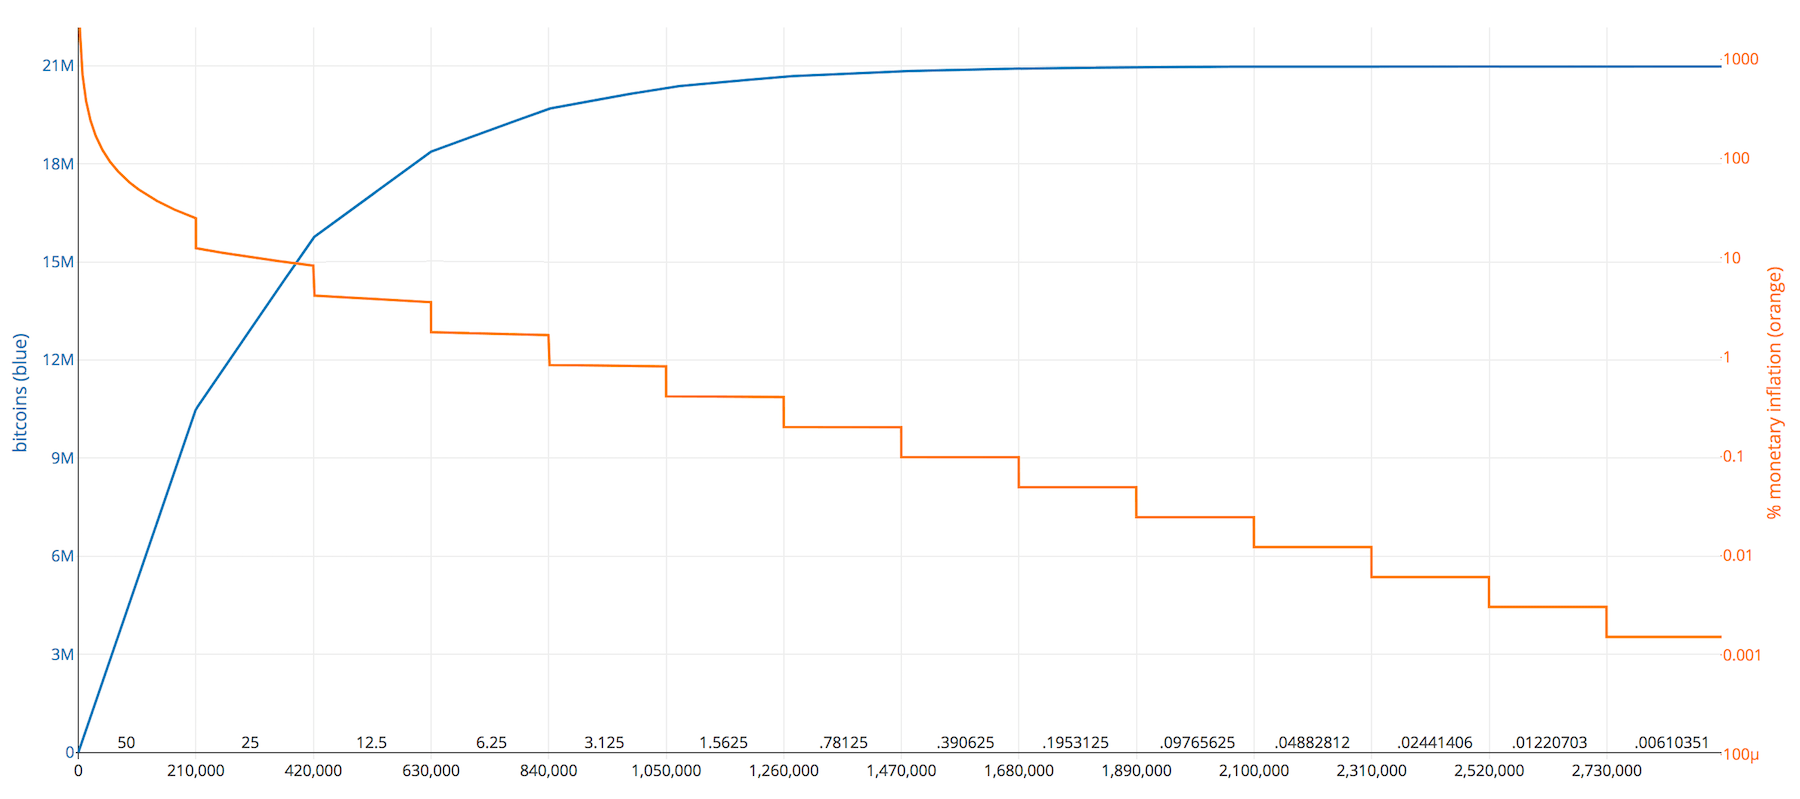
\includegraphics[width = 0.8\textwidth]{rewarding.png}
    \caption{How mining rewarding is planned over time.\cite{rewarding}}
    \label{fig:claim}
\end{figure} 
However, this process is destinated to end, because there is a predetermined number
of coins (21 million) which can spread. To ensure that, every 210.000 blocks 
(corresponding to 4 years), the rewarding given to the creator of the block is halved.
This leads to the second type of incentive in the Bitcoin network: transaction fees.
In fact, for every transaction, there is also a fee amount, which is given to the 
creator of the block as a reward for its effort.




\section{Transactions}
\label{sec:transactions}

To figure out how a transaction works, before it is necessary to understand the concept of
owning a coin. Because, unlike the fiat currency, where you own a physical coin
to spend, owning a bitcoin means that you own the key to unlock the coins from a past
transaction and use them in the new transaction. To get a better sense of the 
transaction mechanism, it is recommended to read a brief extract of the Bitcoin paper: 

"We define an electronic coin as a chain of digital signatures.  Each owner transfers 
the coin to the next by digitally signing a hash of the previous transaction and the 
public key of the next owner and adding these to the end of the coin.  A payee can 
verify the signatures to verify the chain of ownership"\cite{bitcoin}
\begin{figure}[h]
    \centering
    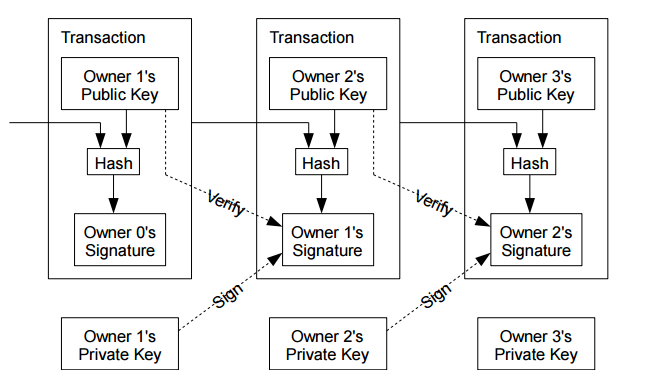
\includegraphics[height=6cm]{bitcoin-transaction.png}
    \caption{Transaction schema. From \cite{bitcoin}}
    \label{fig:trx}
\end{figure}

To go deeper into the design of a transaction, it is useful to imagine a double-entry
ledger. In a few words, every transaction has one or more "inputs"\footnote{debits 
against a bitcoin account.} and one or more "outputs"\footnote{credits added to a bitcoin 
account.}. Usually, outputs add up to slightly less than inputs, because the difference
represents an implied "transaction fee" \ref{sec:incentive}. Higher the fee, higher the 
probability for the transaction to be included in the next block to mine.

Each output, before is spent as an input in a new transaction, waits as an "Unspent
Transaction Output" (UTXO). The sum of all the owned UTXOs, compose the total balance
of a wallet \ref{sec:wallets}.\\
But, not every transaction in the blockchain produces an UTXO.\\ 
Indeed, it depends on 
the scriptPubKey\footnote{A script included in outputs which set the conditions that 
must be fulfilled for those satoshis to be spent. Data for fulfilling the conditions 
can be provided in a signature script (another type of data generated by the spender).}
used into the specific transaction.
\bigskip 
\textbf{Pay To Public Key Hash (P2PKH)} 
Is the most common form of scriptPubKey used to send a transaction to one or multiple 
addresses. In this type of scriptPubKey, the coins sent can be unlocked by a single 
private key corresponding to the public key hashed in the transaction itself. It is 
possible to recognize it by looking at the first character in the address used for the
output. In fact, if it starts with the number "1" it is P2PKH.\cite{bitcoin.org}\pagebreak
\bigskip 
\textbf{Pay To Script Hash (P2SH)}
Was implemented in 2012 to add more flexibility to transactions by adding a hash 
of a second script, the redeem script\footnote{A script similar in function to a 
scriptPubKey. One copy of it is hashed to create a P2SH address (used in an actual 
scriptPubKey) and another copy is placed in the spending signature script to enforce 
its conditions.}. It can be used to process multisignature transactions, 
Open Assets Protocol\footnote{Used to create new currencies upon the Bitcoin blockchain. 
Called colored coins} and to store textual data on the blockchain. The P2SH can 
be recognized by the number "3" at the begin of the addresses.\cite{bitcoin.org}\\

\begin{figure}[h]
    \centering
    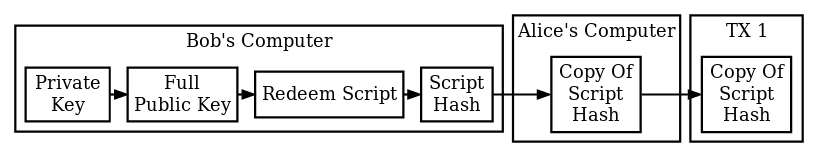
\includegraphics[width = 0.9\textwidth]{p2sh.png}
    \caption{creating A P2SH Redeem Script Hash To Receive Payments \cite{bitcoin.org}}
    \label{fig:p2sh}
\end{figure}\bigskip
\textbf{Multisig}
Are special addresses where to spend a transaction, multiple private keys signature are required.
Although P2SH multisig is now generally used for multisig transactions, this base 
script can be used to require multiple signatures before a UTXO can be spent.
In multisig pubkey scripts, called m-of-n, m is the minimum number of signatures 
which must match a public key; n is the number of public keys being provided.\cite{bitcoin.org}
\bigskip 
\textbf{Null Data}
This type ads arbitrary data to a probably unspendable scritptPubKey that nodes don't have
to store in their UTXOs database. Consensus rules allow null data outputs up to the maximum
allowed scriptPubKey size of 10.000 bytes provided.\cite{bitcoin.org}

\section{Wallets}
\label{sec:wallets}
In simple words, a wallet is the mean through which is possible to manage all the 
owned cryptocurrency. But it can be splitted into two components, programs, and files.
Wallet programs create the public keys to receive the Bitcoin and uses the 
corresponding private key to spend them.\\ 
Wallet files, instead, store the private keys in a file or physically on pieces of paper. 
Furthermore, it also gives the process used for the public-private key creation and 
usage, and  an approach to a deterministic hierarchy key creation process in an unlinkable
keys manner.
\newpage


